\documentclass[mathserif,18pt,xcolor=table]{beamer}
\usepackage{amsmath}
\usepackage{amssymb}
\usepackage{bbm}
\usepackage{ulem}
\usepackage{feynmp-auto}
%\usepackage{slashed}
\usepackage[absolute,overlay]{textpos}
\usepackage{graphicx}
\usepackage{listings}
\usepackage{epsfig}
\usepackage{hyperref}
\usepackage{tikz}
\usetikzlibrary{calc}
\usepackage{enumerate}
%\usepackage{fixltx2e} % buggy
\usepackage[compatibility=false]{caption}
\usepackage{subcaption} % doesn't work with subfigure
%\usepackage{pdfpages}
\usepackage{setspace}
\usepackage{verbatim}
\usepackage{physics}
%\usepackage{siunitx}

\DeclareRobustCommand{\orderof}{\ensuremath{\mathcal{O}}}

\definecolor{dukeblue}{RGB}{0,0,156}
\definecolor{dukedarkblue}{RGB}{0,26,87}
\definecolor{dukeblack}{RGB}{79,79,79}
\definecolor{dukegray}{RGB}{79,79,79}
\definecolor{dukesecbrown}{RGB}{217,200,158}
\definecolor{dukesecblue}{RGB}{127,169,174}
\mode<presentation> {
  \usetheme{Boadilla}  
  \setbeamercovered{invisible}
  \setbeamertemplate{navigation symbols}{}  
  \setbeamertemplate{frametitle}[default][center]
  \setbeamertemplate{bibliography item}{\insertbiblabel}
  \setbeamerfont{frametitle}{series=\bfseries,parent=structure}
  \setbeamerfont{subtitle}{size=\scriptsize,series=\bfseries,parent=structure}
  \setbeamerfont{author}{size=\scriptsize,parent=structure}
  \setbeamerfont{institute}{size=\small,series=\bfseries,parent=structure}
  \setbeamerfont{date}{size=\scriptsize,parent=structure}
  \setbeamerfont{footline}{size=\tiny,parent=structure}
  \setbeamercolor{normal text}{bg=white,fg=dukeblack}
  \setbeamercolor{structure}{fg=dukeblue}
  \setbeamercolor{alerted text}{fg=red!85!black}
  \setbeamercolor{item projected}{use=item,fg=black,bg=item.fg!35}
  \setbeamercolor*{palette primary}{use=structure,fg=white, bg=dukeblue}
  \setbeamercolor*{palette secondary}{use=structure,bg=dukedarkblue,fg=white}
  \setbeamercolor*{framesubtitle}{fg=dukegray}
  \setbeamercolor*{block title}{parent=structure,fg=black,bg=dukeblue}
  \setbeamercolor*{block body}{fg=black,bg=dukeblack!10}
  \setbeamercolor*{block title alerted}{parent=alerted text,bg=black!15}
  \setbeamercolor*{block title example}{parent=example text,bg=black!15}
}

\makeatletter
\setbeamertemplate{footline}{
  \leavevmode
  \hbox{%
    \begin{beamercolorbox}[wd=.333333\paperwidth,ht=2.25ex,dp=1ex,center]{author in head/foot}%
      \usebeamerfont{author in head/foot}\insertshortauthor%
    \end{beamercolorbox}%
    \begin{beamercolorbox}[wd=.333333\paperwidth,ht=2.25ex,dp=1ex,center]{title in head/foot}%
      \usebeamerfont{title in head/foot}\insertshorttitle%
    \end{beamercolorbox}%
    \begin{beamercolorbox}[wd=.333333\paperwidth,ht=2.25ex,dp=1ex,right]{date in head/foot}%
      \usebeamerfont{date in head/foot}\insertshortdate{}\hspace*{2em}%
      \insertframenumber{} / \inserttotalframenumber\hspace*{2ex}%
%      \insertframenumber{} / 11\hspace*{2ex}% TODO hard code to page number before backup!!
    \end{beamercolorbox}}%
  \vskip0pt%
}
\makeatother


\AtBeginSection{\frame{\sectionpage}}


\defbeamertemplate{section page}{mine}[1][]{%
  \begin{centering}
    {\usebeamerfont{section name}\usebeamercolor[fg]{section name}#1}
    \vskip1em\par
    \begin{beamercolorbox}[sep=12pt,center]{part title}
      \usebeamerfont{section title}\insertsection\par
    \end{beamercolorbox}
  \end{centering}
}


\usepackage[protrusion=true,expansion=true]{microtype}
\usepackage{amsmath}
\renewcommand*{\thefootnote}{\fnsymbol{footnote}}
\title[Group Project 1]{Group Project 1\newline Random Walk, Diffusion and Cluster Growth}
\author[Xu, Epland, Li, Cohen]{{\small Yuanyuan Xu, Matthew Epland, Xiaqing Li, Wesley Cohen}}
\institute{Duke University}
%\date{\today}
\date{March 25, 2016}
\hypersetup{
    breaklinks,
    baseurl       = http://,
    pdfborder     = 0 0 0,
    pdfpagemode   = UseNone,% do not show thumbnails or bookmarks on opening
    pdfstartpage  = 1,
    bookmarksopen = true,
    bookmarksdepth= 2,% to show sections and subsections
    pdfauthor     = {\@author},
    pdftitle      = {\@title},
    pdfsubject    = {},
    pdfkeywords   = {}}

\titlegraphic{
\includegraphics[height=2cm]{logos/duke_logo.pdf}}

% Point to nice top level directory
\graphicspath{{../output/plots_for_paper/}}

\begin{document}

\beamertemplateballitem
\frame{\titlepage}
\addtobeamertemplate{frametitle}{}{}


\begin{frame}
  \frametitle{Introduction}
  \begin{itemize}
    \item Bullet point text here TODO
  \end{itemize}

\end{frame}


%%%%%%%%%%%%%%%%%%%%%%%%%%%%%%%%%%%%%%%%%%%%%%%%%%%%%%%%%%%%%%
% Problem 2
%%%%%%%%%%%%%%%%%%%%%%%%%%%%%%%%%%%%%%%%%%%%%%%%%%%%%%%%%%%%%%

\begin{frame}
	\frametitle{Random Walk and Diffusion}
	Suppose $P(i, j, k, n)$ is the probability to find the particle at $(x, y, z)$ at time $t$, then we can get
\begin{equation}
	\scriptsize
	\begin{split}
		P(i, j, k) = \frac{1}{6}[&P(i, j, k, n-1) + P(i-1, j, k, n-1) + P(i, j+1, k, n-1) +\\ &P(i, j-1, k, n-1) + P(i, j, k+1, n-1) + P(i, j, k-1, n-1)].
	\end{split}
\end{equation}
Rearrange this equation and take the continuum limit,
\begin{equation}
	\frac{\partial P(x, y, z, t)}{\partial t} = D\nabla^{2}P(x,y,z,t),
\end{equation}
where $D = (1/6)(\Delta x)^{2} / \Delta t$. 
\end{frame}

\begin{frame}
	\frametitle{Diffusion Equation}
	Suppose the density $\rho$ obeys the diffusion equation,
	\begin{equation}
		\frac{\partial \rho}{\partial t} = D\nabla^{2}\rho.
	\end{equation}
	In one dimension, we have
	\begin{equation}
		\frac{\partial\rho}{\partial t} = D\frac{\partial^{2}\rho}{\partial x^{2}}.
	\end{equation}
	One special solution is
	\begin{equation}
		\rho(x, t) = \frac{1}{\sigma}e^{-\frac{x^{2}}{2\sigma^{2}}},
	\end{equation} 
	where $\sigma$ is time-dependent, with $\sigma = \sqrt{2Dt}$. 
\end{frame}

\begin{frame}
	\frametitle{$\expval{x^{2}(t)}$ of 1D Normal Distribution}
	The formula for computing the expectation value is given by
	\begin{align}
	\expval{x^{2}(t)} &= \int_{-\infty}^{+\infty} \rho(x, t) x^{2} dx, \\
	\expval{x^{2}(t)} &= \frac{2}{\sqrt{2\pi\sigma^{2}(t)}} \int_{0}^{+\infty} x^{2} \exp(-\frac{x^{2}}{2\sigma^{2}(t)}).
\end{align}
Now we use the Gaussian integral that
\begin{equation}
	\int_{0}^{+\infty} x^{2n} \exp(-x^{2}/a^{2}) dx = \sqrt{\pi} \frac{(2n)!}{n!}\Big( \frac{a}{2} \Big)^{2n+1}.
\end{equation}
Let $n = 1$ and $a = \sqrt{2}\sigma(t)$, we can get
\begin{equation}
	\begin{split}
		\expval{x^{2}(t)} &= \frac{2}{\sqrt{2\pi\sigma^{2}(t)}} \cdot \sqrt{\pi}\cdot \frac{2!}{1!} \cdot \Big( \frac{\sqrt{2}\sigma(t)}{2} \Big)^{3} \\
		&= \sigma^{2}(t).
	\end{split} 
\end{equation}
\end{frame}

\begin{frame}
	\frametitle{Numerical Methods}
	\begin{itemize}
		\item Set spatial and time step size
		\begin{itemize}
		\item
		$\Delta x = 0.05, \Delta t = 10^{-4}, D = 2$ which satisfy $\Delta t \leq (\Delta x)^{2}/(2D)$
		\end{itemize}
		\item Set boundary conditions
	    \begin{itemize}
	    \item
	    	$\rho(-5) = \rho(5) = 0$
	    \end{itemize}
	    \item Set initial conditions
	    \begin{itemize}
	    	\item $\rho(x) = \begin{cases}
	    	1/3 & x = -\Delta x, 0, \Delta x \\
	    	0 & \mathrm{others}\\
	    	\end{cases}$
	    \end{itemize}
	    \item Loop over time steps and spatial steps
	    \begin{itemize}
	    	\item {
	    	\tt
	    	for i in range(t\_max): \\
	    	\qquad for j in range(size):\\
	    	\qquad \qquad $\rho$[j] += D*dt*($\rho$[j+1] - 2*$\rho$[j] + $\rho$[j-1])/dx$^{2}$
	    	}
	    \end{itemize}
	    \item Perform a fit for 5 different time snapshots
	\end{itemize}
\end{frame}

\begin{frame}
	\frametitle{Snapshots}
	\begin{figure}
  	\centering
  	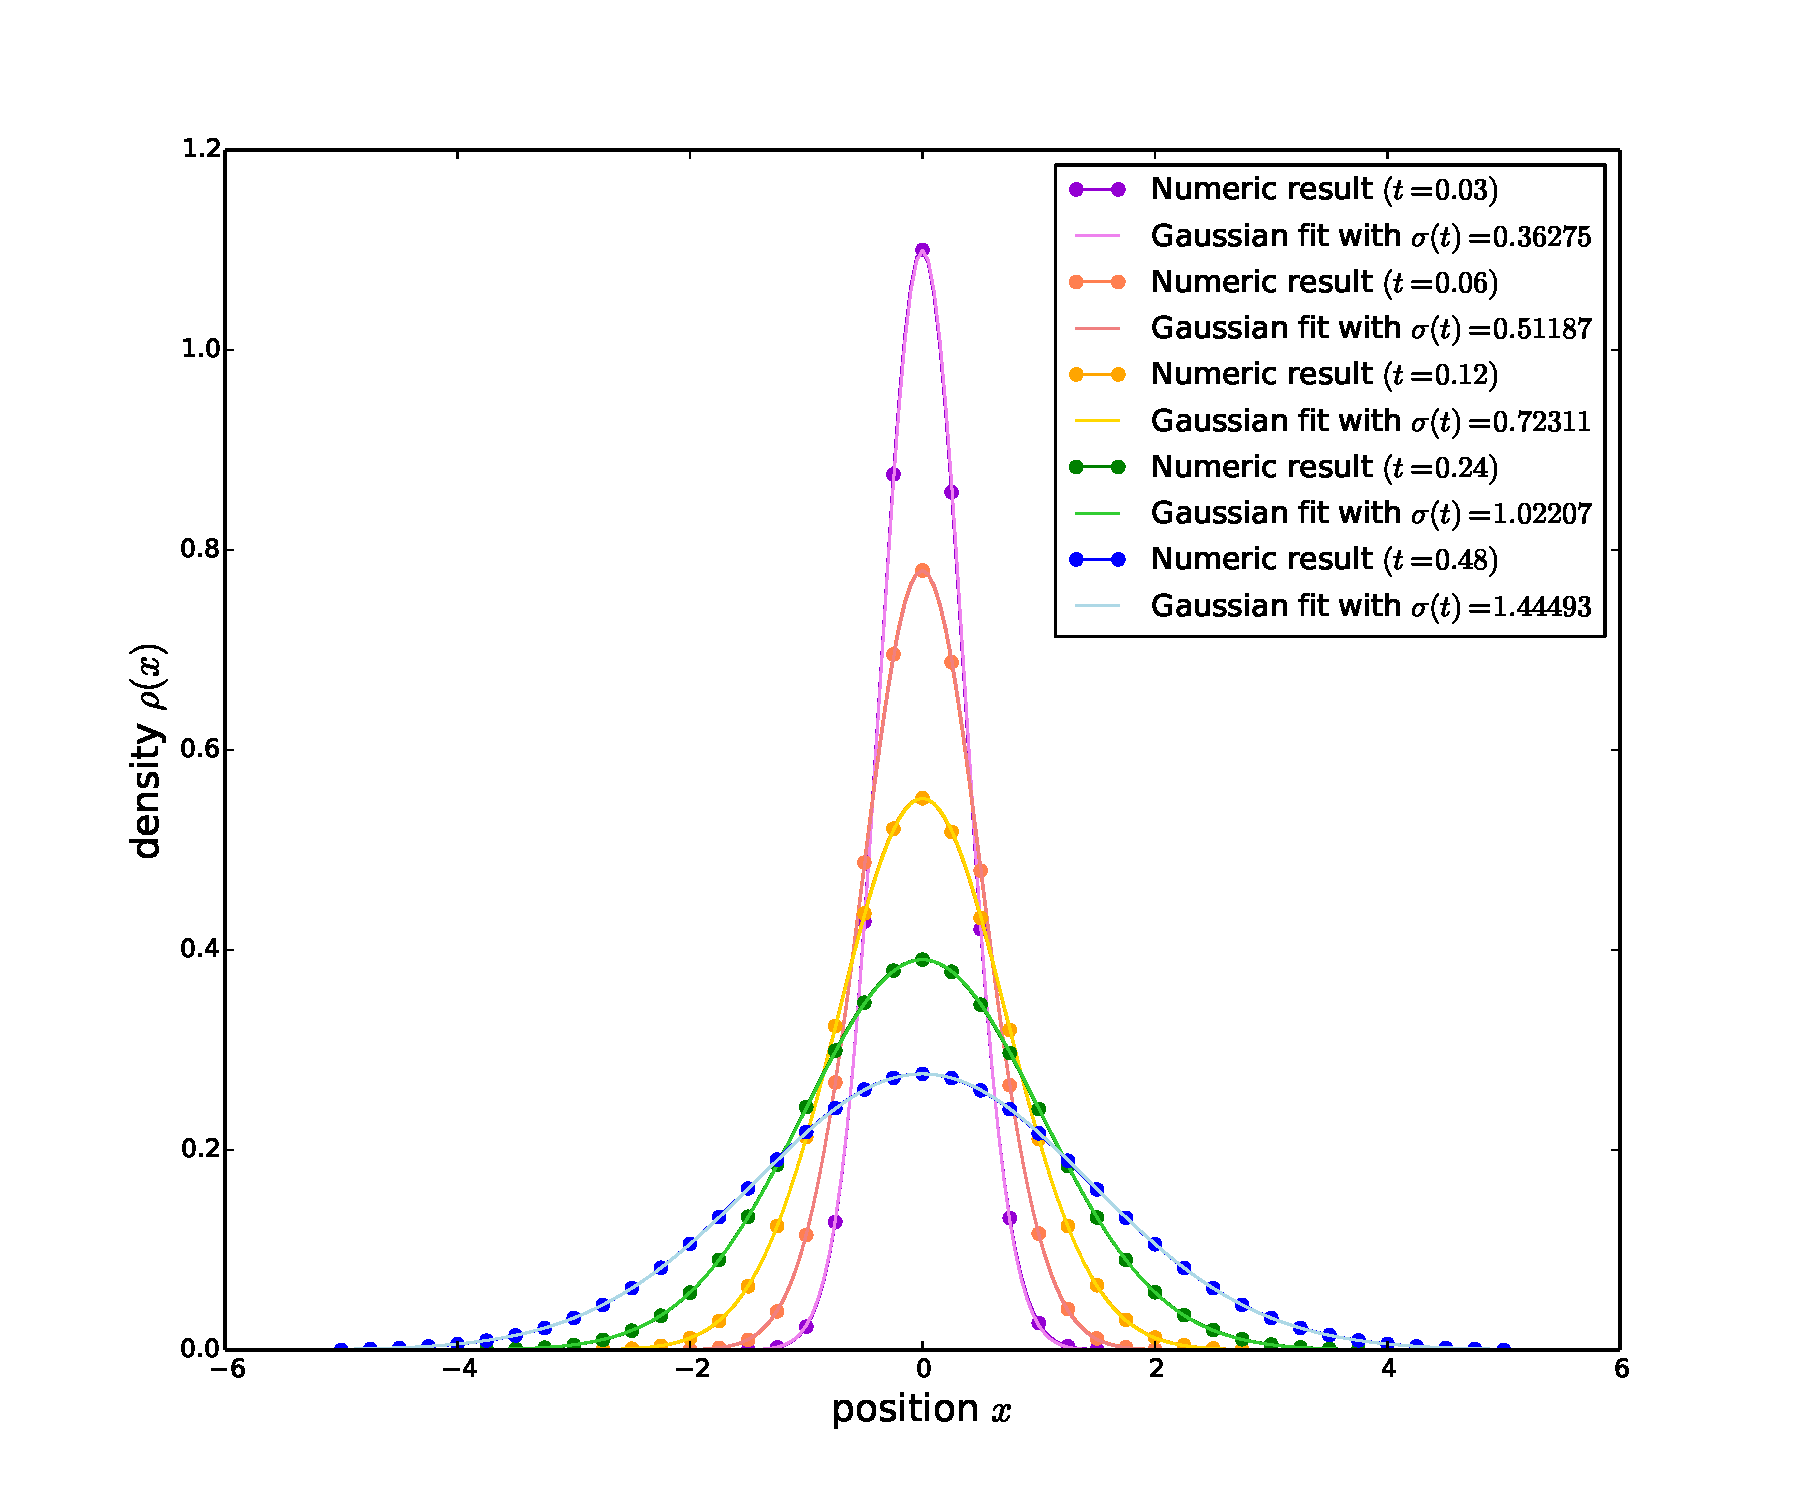
\includegraphics[width=0.85\textwidth]{../output/plots_for_paper/problem_2/part_b.pdf}
\end{figure}
\end{frame}

\begin{frame}
	\frametitle{Verification}
	\begin{center}
	\begin{tabular}{ | p{1.5cm} | p{1.5cm} | p{2.5cm} | p{2cm} | p{2.5cm} |}
		\hline
		Steps & Time & $\sigma(t) = \sqrt{2Dt}$ & $\sigma_{\mathrm{fit}}(t)$ & Percent error\\
		\hline
		300  & 0.03 & 0.346410 & 0.362748 & 4.716236\%\\
		\hline
		600  & 0.60 & 0.489898 & 0.511874 & 4.485857\%\\ 
		\hline
		1200 & 1.20 & 0.692820 & 0.723106 & 4.371316\%\\
		\hline
		2400 & 2.40 & 0.979796 & 0.102207 & 4.314208\%\\
		\hline
		4800 & 4.80 & 0.138564 & 0.144493 & 4.278783\%\\
		\hline
	\end{tabular}
\end{center}
\begin{itemize}
	\item $\sigma(t) = \sqrt{2Dt}$
	\item $\expval{r^{2}} \propto t$
\end{itemize}
\end{frame}


%%%%%%%%%%%%%%%%%%%%%%%%%%%%%%%%%%%%%%%%%%%%%%%%%%%%%

\begin{frame}
  \frametitle{DLA Cluster: RNG Seed $= 6$}
\begin{figure}
  \centering
  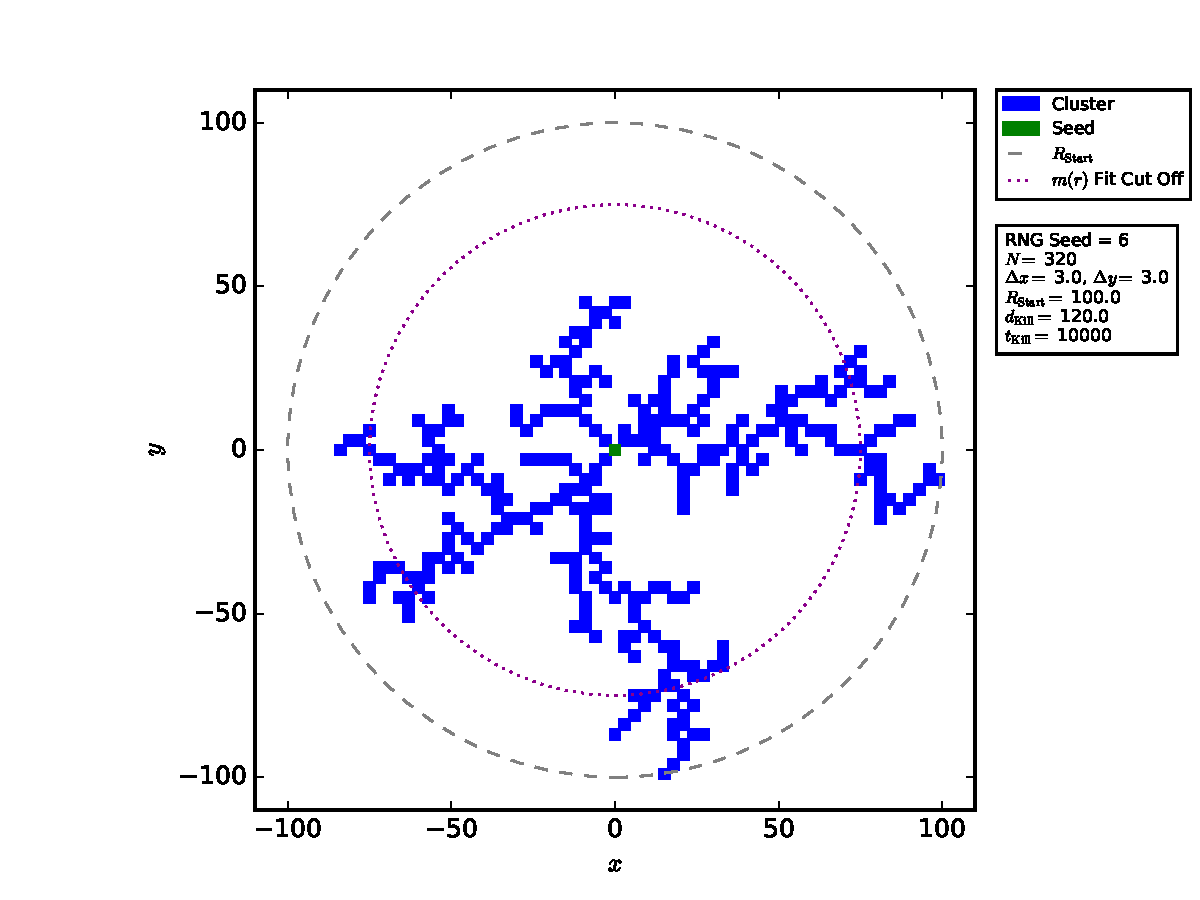
\includegraphics[width=0.9\textwidth]{problem_3/large_cluster_seed_num_6.pdf}
\end{figure}
\end{frame}

\begin{frame}
  \frametitle{DLA Cluster Mass: RNG Seed $= 6$}
\begin{figure}
  \centering
  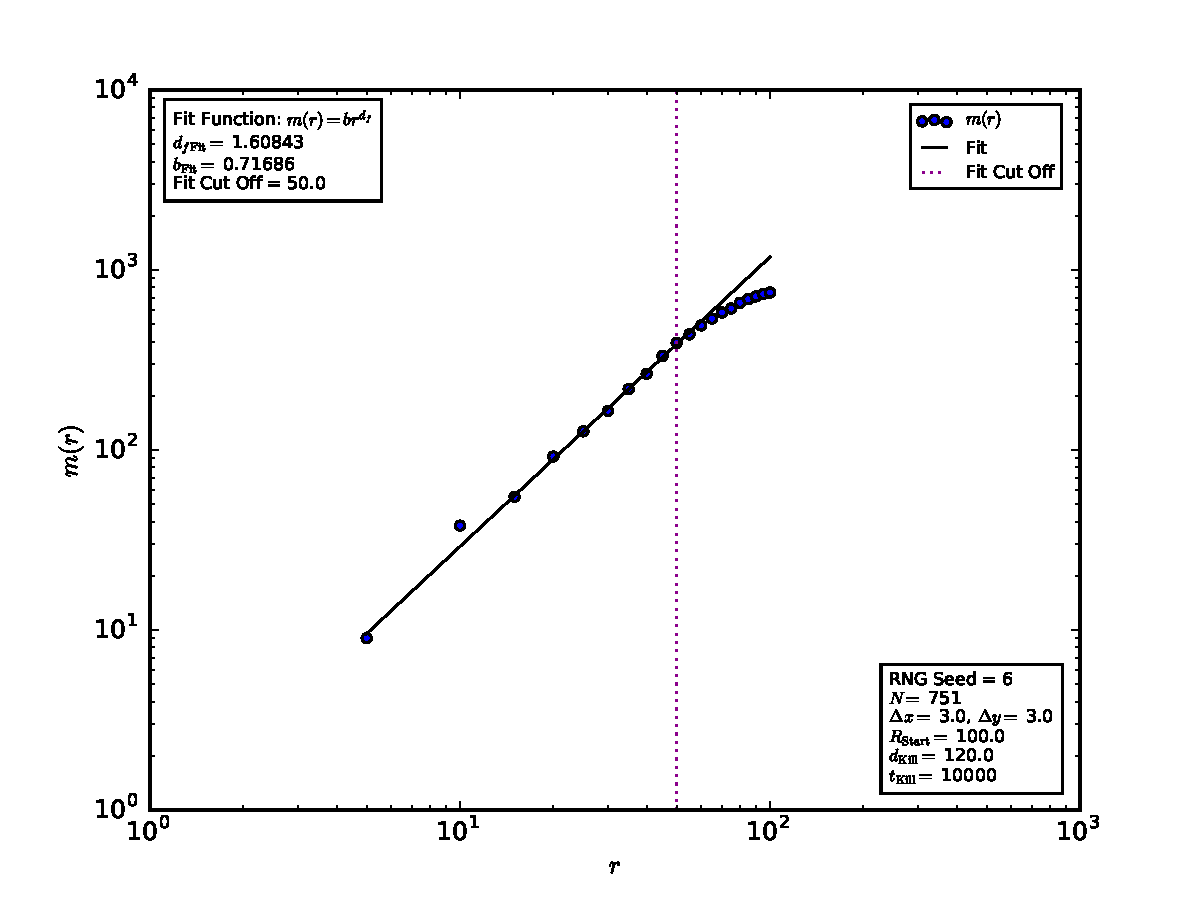
\includegraphics[width=0.9\textwidth]{problem_3/large_cluster_mass_seed_num_6.pdf}
\end{figure}
\end{frame}

\begin{frame}
  \frametitle{DLA Cluster: RNG Seed $= 10$}
\begin{figure}
  \centering
  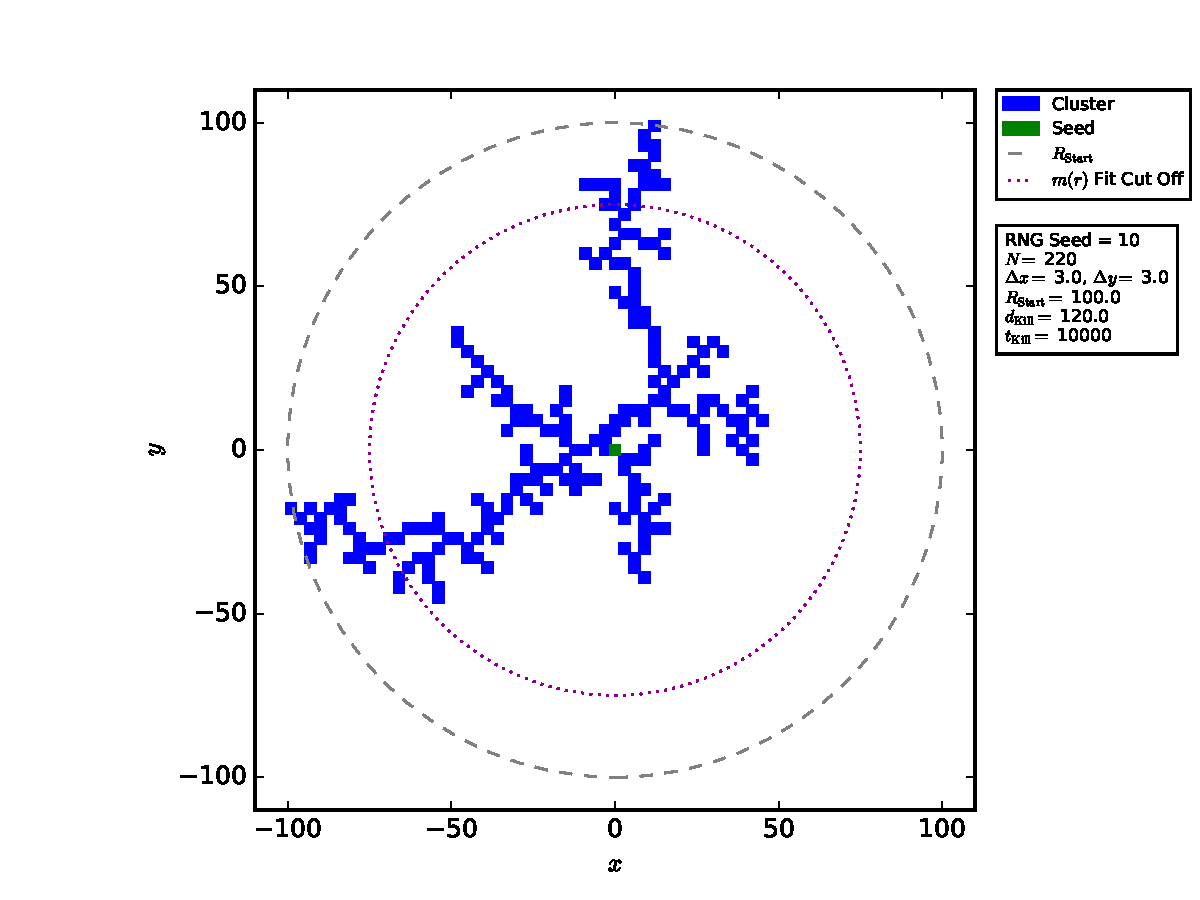
\includegraphics[width=0.9\textwidth]{problem_3/large_cluster_seed_num_10.pdf}
\end{figure}
\end{frame}

\begin{frame}
  \frametitle{DLA Cluster Mass: RNG Seed $= 10$}
\begin{figure}
  \centering
  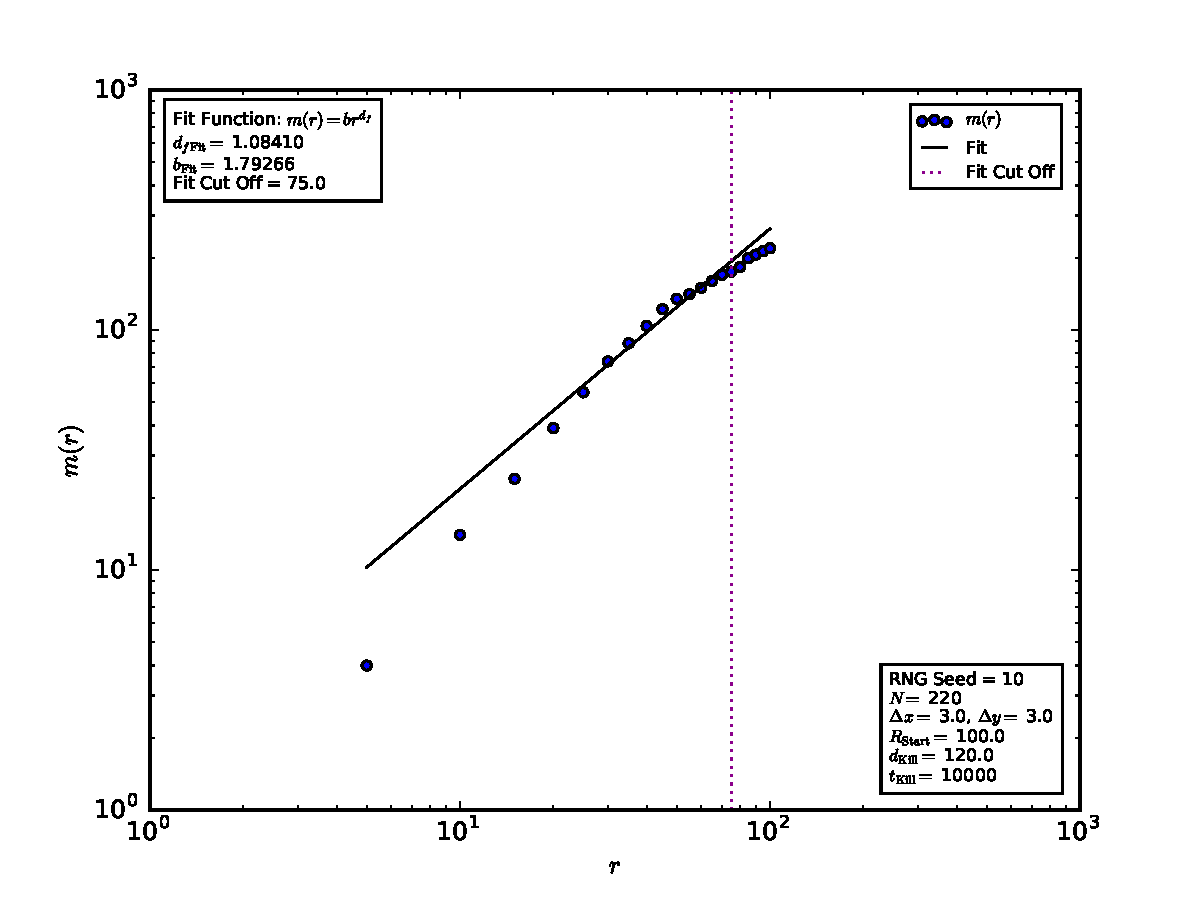
\includegraphics[width=0.9\textwidth]{problem_3/large_cluster_mass_seed_num_10.pdf}
\end{figure}
\end{frame}

\begin{frame}
  \frametitle{DLA Cluster: RNG Seed $= 12$}
\begin{figure}
  \centering
  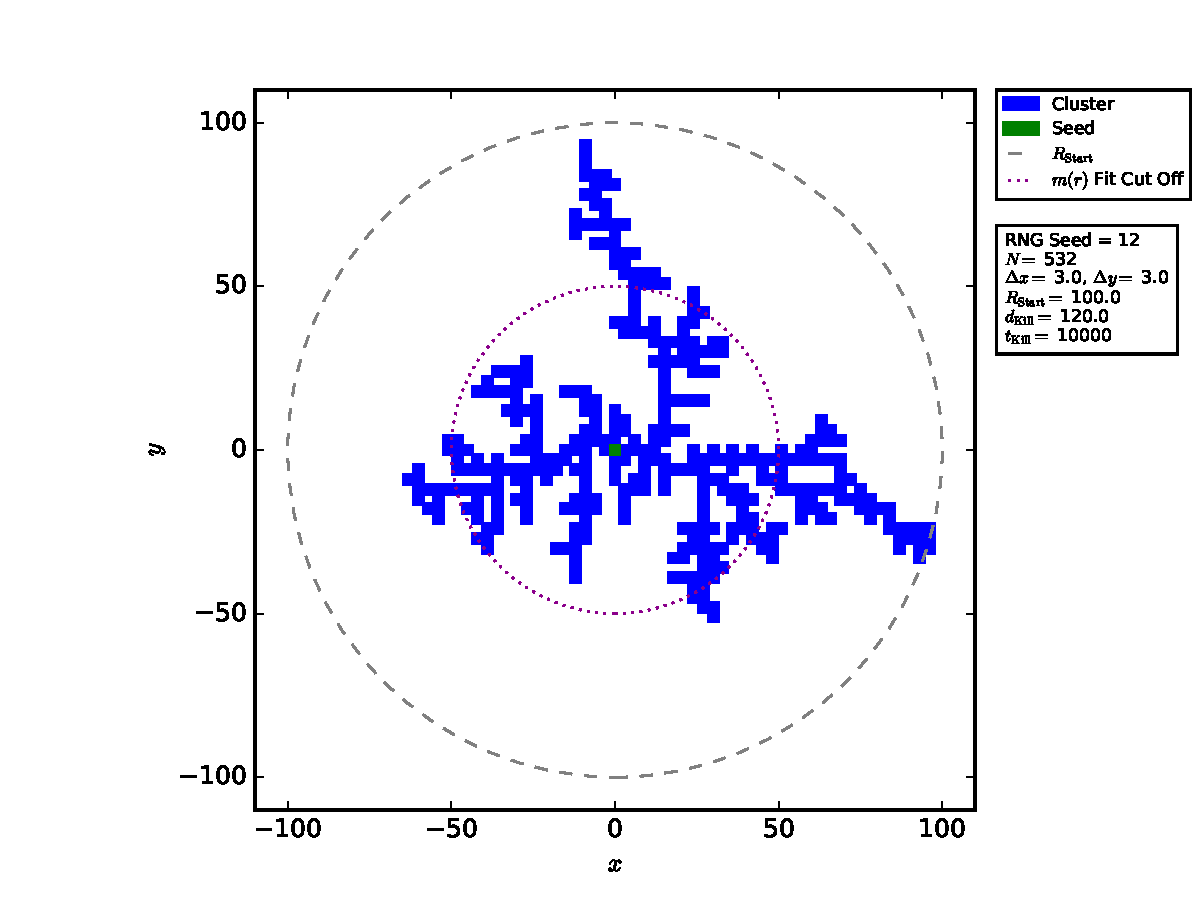
\includegraphics[width=0.9\textwidth]{problem_3/large_cluster_seed_num_12.pdf}
\end{figure}
\end{frame}

\begin{frame}
  \frametitle{DLA Cluster Mass: RNG Seed $= 12$}
\begin{figure}
  \centering
  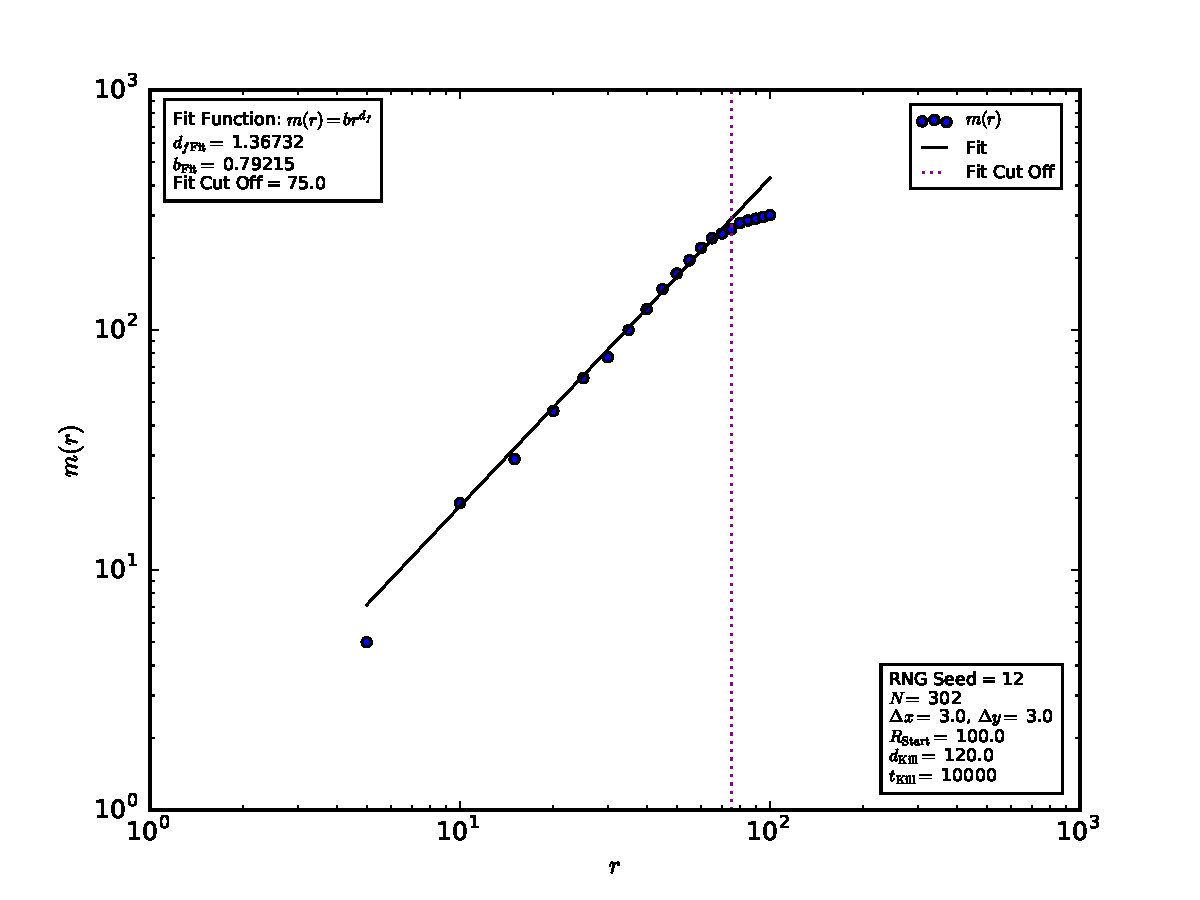
\includegraphics[width=0.9\textwidth]{problem_3/large_cluster_mass_seed_num_12.pdf}
\end{figure}
\end{frame}

\begin{frame}
  \frametitle{Fractal Dimensionality}

  \begin{itemize}
    \item Running over 10 different RNG seeds we find:
    \begin{itemize}
      \item $\left<d_{f}\right> = 1.30$, with Std. Dev. $= 0.10$ 
    \end{itemize}
  \end{itemize}

% You can position text/figures/anyting at an arbitrary position with textblock*
\begin{textblock*}{0.9\textwidth}(1.4cm,8.5cm) % {block width} (coords) note coords are from upper left corner
{\tiny All $d_{f\,\mathrm{fit}} = 1.3347,\,1.3463,\,1.4241,\,1.3854,\,1.0841,\,1.3420,\,1.3673,\,1.2641,\,1.2410,\,1.1970$}
\end{textblock*}

\end{frame}


\end{document}
%%%%%%%%%%%%%%%%%%%%%%%%%%%%%%%%%%%%%%%%%%%%%%%%%%%%%%%%%%%%%%%%%%%%

% Backup
\begin{frame}
    \begin{center}
    \usebeamerfont{frametitle}Backup
    \end{center}
\end{frame}

% bib
\begin{frame}%[allowframebreaks]
        \frametitle{References}
	\bibliographystyle{../bib_files/atlasBibStyleWoTitle}
{\scriptsize
        \bibliography{../bib_files/my_bib.bib}
}
\end{frame}


